\chapter{Maximum Likelihood Estimator}
\label{ch:MLE}
\section{Overview}
The path of the Cosmic Microwave Background (CMB) photons gets bent due to the intervening galaxy cluster. 
Distortion in the background CMB is of the order of few arcminutes for a massive galaxy cluster.
On the galaxy cluster length scales (order of arcminutes) CMB can be approximated as a gradient due to diffusion damping \citep{silk96}. 
Gravitational lensing induces a dipole kind of structure on top of the gradient with hot and clod spots swapped. 
The strength of the gravitational lensing signal (lensing dipole) is directly proportional to the background gradient and the cluster mass. 
As polarisation signal is an order of magnitude smaller than temperature, lensing signal in polarisation is also an order of magnitude smaller than that of temperautre. 
Fig ~\ref{fig:lensing_signal} shows the lensing signal for a cluster of mass $5*10^{14}$ $M_{\odot}$ and at redshift of $z$ = 0.7.
On the left panels we have the background CMB gradient for the temperature and polarisation stokes Q and U parameters, on the middle panel we have the corresponding lensed maps; on the right panel we have the lensing dipole signatures.

Lensing remaps the unlensed CMB temperature and polarisation fields based on the gravitational deflection angle of the cluster. 
\begin{eqnarray}
T(\hat{n}) = \tilde{T}(\hat{n} + \alpha(\hat{n}))\\
Q(\hat{n}) = \tilde{Q}(\hat{n} + \alpha(\hat{n}))\\
U(\hat{n}) =  \tilde{U}(\hat{n} + \alpha(\hat{n}))
\end{eqnarray}
where T represents the temperature field, Q and U are the stokes polarisation parameters respectively. 
Tilde represents the unlensed fields, $\alpha(\hat{n})$ is the deflection angle vector due to the cluster lensing along the $\hat{n}$ direction. 
Deflection angle is related to gravitational potential as $\nabla \phi (\hat{n})$ and is directly proportional to the mass of the cluster.

In literature, there are several methods to extract lensing singal from CMB data. 
During my thesis, I mainly worked on two methods for extracting lensing signal from the observed CMB data: Maximum Likelihood Estimator (MLE) and Quadratic Estimator (QE). 
In this chapter, I will explain the MLE in detail. While we compare the results of MLE with QE, QE is explained in detail in next chapter.
\begin{figure}[ht]
\begin{center}
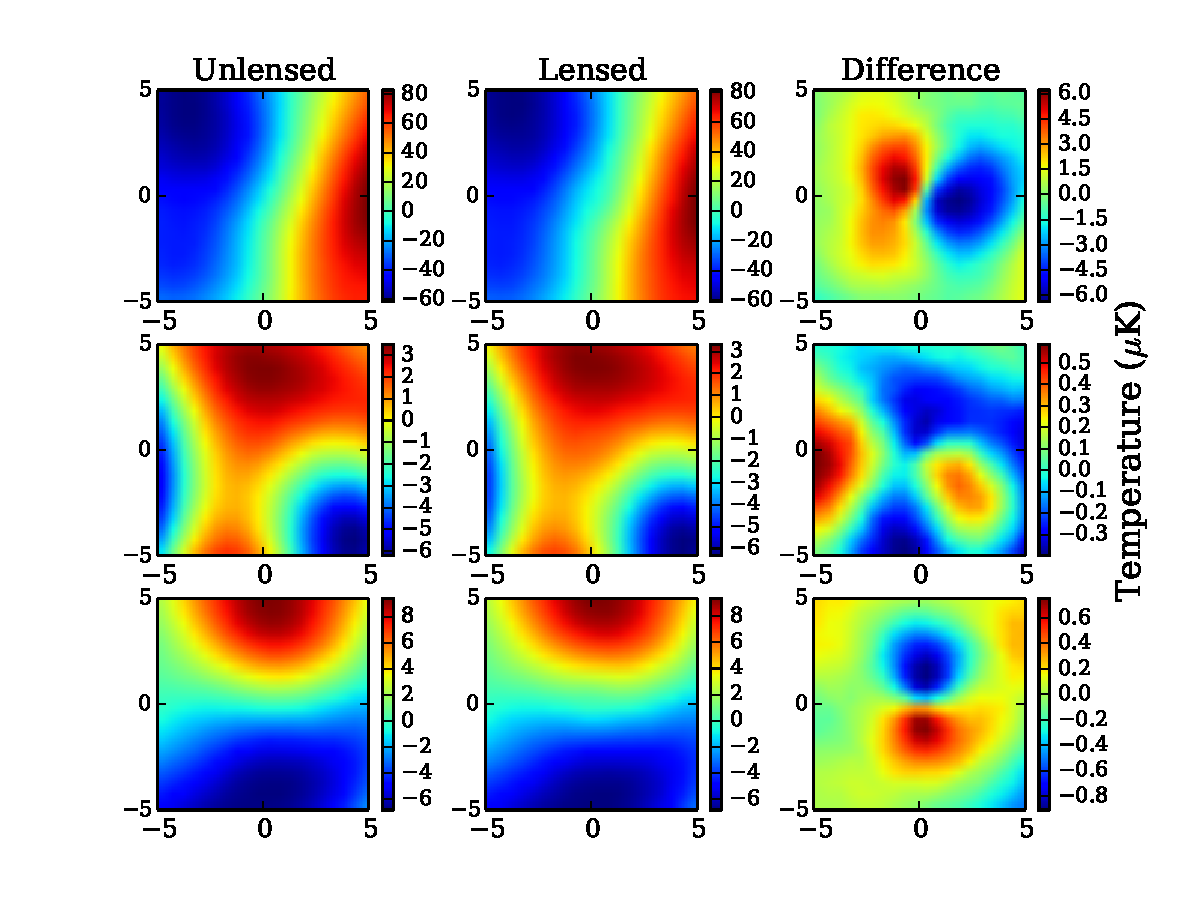
\includegraphics[width=\linewidth, keepaspectratio]{figs/lensing_signal.pdf}
 \caption{Lensing effect on CMB due to a galaxy cluster of mass $5\times 10^{14}$ \msolar.
  On the top panel we show the effect of cluster lensing on CMB temperature field.
  Bottom two panels are for the stokes Q and U parameters. 
 } 
\label{fig:lensing_signal}
\end{center}
\end{figure}

\section{Maximum Likelihood Estimator}
\label{sec_MLE}
Gravitational lensing by a galaxy cluster induces extra pixel-pixel correlations. 
MLE extracts the lensing signal by modeling these pixel-pixel correlations in the form of covariance matrix.


\subsection{Covariance matrix calculation}
Here, I explain the calculation of covariance matrix which will act as the model.
The distortion of CMB due to a galaxy cluster is of the order of arcminutes; much of the lensing is within 10\am from cluster center.
For covariance matrix calculation we take central \smallboxsize cutout.
We also checked that by increasing the boxsize to 14\am we gain an improvement in a SNR of less than 1\%, however, that the increases the computational complexities. 


 We calculate the covariance matrix by using a set of simulated skies. 
 To calculate the simulated lensed CMB sky, first we generate the large-scale structure lensed CMB power spectra ($C^{TT}_{l}, C^{TE}_{l}, C^{EE}_{l},$ and $C^{BB}_{l}$) form CAMB for the $planck$ 2015 cosmology \citep{planck15_13}.  
 We generate Gaussian random realisations with these power spectra on a 50\am X 50\am box. 
 Q and U maps are generated by using E and B maps as
 \begin{eqnarray}
Q = E + B\\
U = E + B
 \label{eq:coord_trans}
 \end{eqnarray}
 
 \pending{correct the equations}
 While we only use  \smallboxsize  for final calculations we simulate a bigger box (50\am) to take into account the large scale gradient.
 These Gaussian realizations are then lensed by an assumed galaxy cluster density profile (explained in next section). 
 
 With simulated lensed CMB maps in hand we calculate the covariance matrix as follows
 \begin{eqnarray}
\Sigma_{lens}(M,z) & = & \left<(\textrm{\textbf{G}} - \left<\textrm{\textbf{G}}\right>) (\textrm{\textbf{G}} - \left<\textrm{\textbf{G}}\right>)^{T}\right>\\
  =   \frac{1}{n-1}\sum\limits_{i = 0}^{n} (\textrm{\textbf{G}}_{i} - \left<\textrm{\textbf{G}}\right>) (\textrm{\textbf{G}}_{i} - \left<\textrm{\textbf{G}}\right>)^{T} %(\textrm{\textbf{G}}_{i} - \left<\textrm{\textbf{G}}\right\
%s>)^{T},
\label{eq_lensed_cmb_cov_mass_z}
\end{eqnarray}
 where vector $G_{i}$ is either the polarisation or temperature simulated data for $i^{th}$ sky realisation. 
 The number simulated skies depend on the number of degrees of freedom in the covariance matrix. 
 In our case, we concatenate Q and U maps for our polarisation estimator for which the covariance matrix is a 800 X 800 matrix. 
 Number of simulations scale as twice the number of elements in the covariance matrix; we found 1,30,000 simulations are sufficient for recovering cluster masses without any bias. 
  We then multiply Hartlap correction term $\frac{(n_{sims} -n_{d} -1)}{n_{sims}}$, where $n_{sims}$ is 1,30,000 and $n_{d}$ is the length of the vector 400(800) for T(QU), to remove any possible bias in $\Sigma^{-1}_{lens}$ due to the limited number of simulations. 
  
 We also use these simulated skies to quantify the effects of statistical and systematic uncertainties.
 There are several astrophysical sources which act as a systematic bias and foregrounds for the CMB-cluster lensing analysis. 
 In this work we consider clusters own SZ effects such as thermal Sunayev-Zel'dovich (tSZ) and kinematic Sunayev-Zel'dovich effects. 
 %tSZ is in explained in detail in the next chapter. 
 Along with these SZ effects we have also considered sources which are uncorrelated with cluster such as tSZ effect from other halos, dusty star forming galaxies (DSFGs), and radio galaxies.
 In appendix, we provide in more details about the addition of these foregrounds to simulated skies.
 
 In this chapter we have considered only simulated data to check the efficiency of MLE. 
 Unless otherwise mentioned all the clusters are simulated at a mass of $M_{200} = 2*10^{14}$\msolar \pending{footnote} and at redshift of 0.7.
 For covariance matrix calculation we simulate the skies at redshift of $0.7$ with mass resolution of $2*10^{12}$\msolar. 
 Note that such fine gridding might not be computationally feasible for data where the clusters span wide range of masses and redshifts.
 An optimal solution would be generate the covariance matrices on coarser grid of mass and redshift and then interpolating it on a finer grid.
 
 
 
  
   
  
  \subsection{Likelihood Estimation}
  With the covariance matrix in hand we calculate the likelihood given the data as follows 
  
  \begin{equation}
  -2lnL(d|\Sigma_{lens}) = ln |\Sigma_{lens}| + d^{T} \Sigma^{-1}_{lens} d
  \end{equation}
  where the data vector $d$ is the pixel values of the observed T or Q/U maps.
  The pixel values are defined as the variations from the mean CMB temperature (polarisation) and hence have zero mean.
  
  %Since the majority of the lensing singal is within few arcminutes from the cluster center, we carry out the lensing analysis within \smallboxsize of the cluster center to simplify and speed up the analysis. 
  %We also checked that by increasing the boxsize to 14\am we gain an improvement in a SNR of less than 1\%, however, that the increases the computational complexities. 
  As pointed out earlier, the lensing signal of a single galaxy cluster is much weaker to be detected. 
  We stack many clusters to increase SNR (signal to noise ratio) to a reasonable level
  \begin{equation}
  -2ln L(d| \Sigma_{lens})_{tot} = \Sigma^{n}_{i =0} w_{i} [ln |\Sigma_{lens}| + d^{T}_{i} \Sigma^{-1}_{lens}  d]
  \end{equation}
  where n is the total number of clusters in the sample, $w_{i}$ is the weight for the $i^{th}$ cluster which depends on the survey noise etc.. 
  In this chapter as we are using simulated clusters, we assign uniform weights to each cluster.  

  \subsection{Lensing convergence profile}
  In order to lens the simulated CMB sky we need to know the lensing deflection angle.
  Deflection angle depends on the lensing convergence profile as follows:
\begin{equation}
 \alpha = \nabla. k = -\nabla^{2} \phi
 \end{equation}
 where $\alpha$ is the deflection angle, $k$ is the lensing convergence profile, and $\phi$ is the lensing potential.
 For a symmetrical density profiles, the lensing convergence profile is equal to the ratio of surface mass density over the critical density of the Universe at the cluster redshift $k = \frac{\sigma(x)}{\sigma_{crit}}$.
 
The surface mass density or also know as the projected mass density of the halo is obtained by integrating the halo density profile along the line of sight. 
 \begin{equation}
 \sigma(x) = 2 \int^{\inf}_{0} \rho(r) ds
 \label{eq:surface_density}
 \end{equation}
 where r is the radial distance, x is the corresponding 2D planar distance and s is distance along the line of sight with s =0 being the plane of the cluster.
 The critical surface density of the Universe at cluster redshift is given by
 \begin{equation}
 \sigma_{crit} = \frac{c^{2}}{4\pi G} \frac{D_{cmb}}{D_{clus}D_{cmb,clus}}
 \end{equation}
 where $D_{cmb}$ is the comoving distance to the epoch of recombination (z= 1100), $D_{clus}$ is the comoving distance to the cluster (in our case comoving distance to the redshift), and $D_{cmb,clus}$ is the comoving distance between the CMB and the cluster.
 
 Unless otherwise mentioned, I define all the cluster quantities in the chapter with respect to $R_{200}$, which is defined as the radius within which the mean cluster density is 200 times the Universe critical density at cluster redshift $\rho^{z}_{crit}$. $M_{200}$ will be 
 \begin{equation}
 M_{200} = \int^{R_{200}}_{0}  4\pi x^{2} \rho(x) dx
 \end{equation}
 By definition $M_{200}$ is also given by
 \begin{equation}
 M_{200} = \frac{800\pi}{3} R^{3}_{200} \rho^{3}_{crit}
 \end{equation}
 
 The above mathematical equations hold for any spherically symmetric halo, now we move on to a specific case of Navarro Frenk White (NFW) halo density profile.
 In the NFW profile, the density of the dark matter halo as function radius is given by:
 \begin{equation}
 \rho(r)= \frac{\delta_{c}\rho^{z}_{crit}}{(\frac{r}{R_{s}})(1+\frac{r}{R_{s}})^{2}}
 \end{equation}
 where $\delta_{c}$ is the characteristic over-density, $R_{s}$ is the characteristic scale radius, and $c$ is the dimensionless concentration parameter.
 The dimensionless over-density is given by $\delta_{c} = \rho_{0}/\rho^{z}_{crit}$, where $\rho_{0}$ is the cluster central density and  $\rho^{z}_{crit}$  is the crititcal density of the universe at cluster redshift.
 Plugging the above equation in ~\ref{eq:surface_density}, we get the surface density for the NFW halo. 
 By slightly change the variables of integration as $s=\sqrt{r^{2} - x^{2}}$ and $ds = \frac{rdr}{\sqrt{r^{2} - x^{2}}}$ we obtain:
 \begin{equation}
 \Sigma(x) = 2\delta_{c} \rho^{z}_{crit} R^{3}_{s} \int^{\inf}_{x} \frac{1}{r(R_{s} + r)^{2}} \frac{rdr}{\sqrt{r^{2} - x^{2}}}
 \label{eq:sr_den}
 \end{equation}
 The scale radius is related to the concentration parameter as follows:
 \begin{equation}
 c = \frac{R_{200}}{R_{s}}
 \end{equation}
 In this chapter we have set $c = 3.0$ following \cite{bhattacharya13}.
 The ~\ref{eq:sr_den} can be solved analytically and the explicit closed-form expression for the NFW case has been given by \cite{bartelmann96}.
 Unless otherwise mentioned we consider the galaxy clusters to follow NFW profile, however,  the mathematical framework described above can be applied any halo density profile. 
 
 
 \section{Results}

 In this section first we validate our pipeline using simulations, we report the expected mass uncertainties for the polarisation and temperature MLE. 
 Then we compare the performance of MLE and QE for ideal simulations by only vary the experimental noise levels and not including any galactic or extra galactic foregrounds. 
 Later, we compare the performance of the estimators in the presence of foregrounds. 
 In this chapter all the results are for a set of 100,000 simulated clusters (expected number of clusters for CMB-S4) each at a mass of $2\times10^{14} M_{\odot}$ and at redshift of 0.7.
 To obtain the lensing significance, we calculate the ratio of combined likelihood at zero mass to that of maximum likelihood:
 \begin{equation}
 \lambda = \frac{L (M_{200} =0)}{max(L(M_{200}))}
 \end{equation} 
 According the Wilk's theorem, in many cluster limit $\lambda $ follows chi-square statistic with one degree of freedom ($M_{200}$ in our case).
 The detection significance reported in this chapter is equal to $-2 ln (\chi)$
 Similarly, we obtain the errors on mass estimate by calculating masses at which $-2lnL(M_{est}) + 2 ln L (M_{200})$ is equal to 1, where $M_{est}$ is the best fit mass.
 
 
 \subsection{Ideal simulations}
 There are two main purposes for our ideal simulations. 
 Firstly, ideal simulations serve as benchmark to estimate the effect of different systematic and statistical sources of uncertainties on our lensing analysis. 
 In addition to that, it provides equivalent conditions to allow for a fair comparison between MLE and QE.
 To validate the pipeline we simulated 100,000 galaxy clusters each at a mass of $2*10^{14} M{\odot}$ and at redshift of $z = 0.7$; later we added white noise realisation at 1\ukam.
 In the top panel of Fig 1, the black solid line represents the combined likelihood for temperature MLE estimator, solid orange curve is that for the polarisation QU estimator and the dashed orange curve is for EB estimator. 
 We calculated the detection significance as mentioned above, lensing signal detected at 400$\sigma$ and 110$\sigma$ for temperature and polarisation MLE respectively. 
 Null test results are shown in bottom panel of Fig. 1, for which we turned of lensing in our pipeline.
 As expected for all the three MLE estimators (T, QU, and EB) the likelihoods peak at zero mass.
 
 \begin{figure}
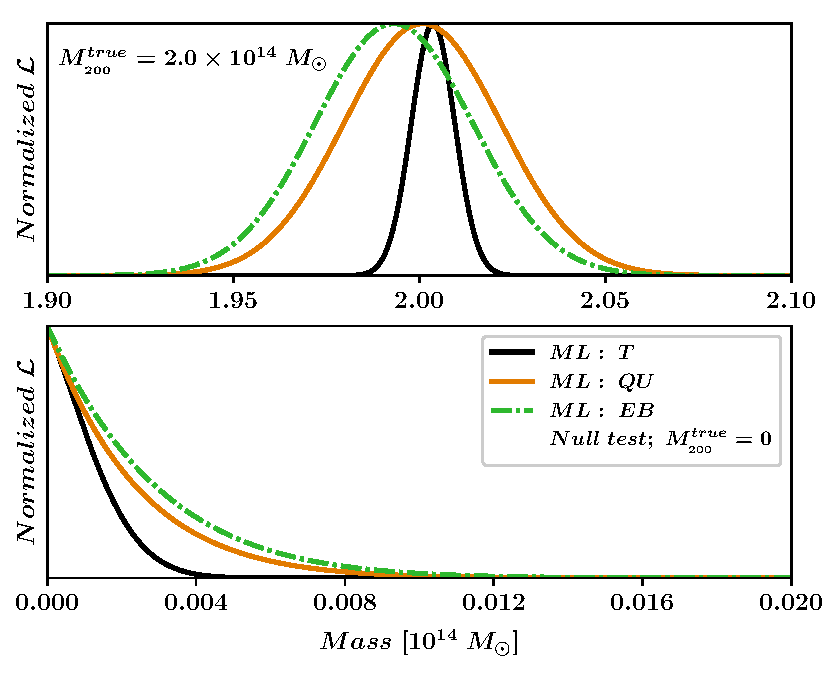
\includegraphics[width=\linewidth, keepaspectratio]{figs/fig0-eps-converted-to.pdf}
 \caption{In the top panel we show the combined likelihood of 100,000 clusters each at redshift of 0.7 and at mass of $2\times 10^{14} M_{\odot}$ for temperature and polarisation MLE estimators. The difference between QU and EB estimator isn't statistically significant. In the bottom panel we show the results of null test and as expected the likelihood peaks at zero for all three estimators}
 \end{figure}
 
 In the left panel of figure 2., we compare the performances of all three MLE estimators and the temperature QE estimator as function of experimental noise levels. 
 %Note that, no galactic or extra galactic foregrounds are added. 
 %All the fractional mass uncertainties are stated for 100,000 clusters each at a mass of $2\times 10^{14} M_{\odot}$ and at a redshift of 0.7.
 It is evident from the figure that in the absence of foregrounds, temperature outperforms polarisation above noise-level of 0.075 \ukam.
 So even for future CMB-S4 experiment temperature has to be the primary channel from pure SNR perspective.
 Only below noise-level of  0.075 \ukam, polarisation starts competing with temperature.
 As pointed out earlier, the lensing signal is directly proportional to the background CMB gradient, gradient in polarisation is 10$\times$ smaller than that of temperature as shown in ~\ref{fig:lensing_signal}. However, below noise-level of 0.075\ukam the CMB temperature background gradient acts as a source of noise. 
 
 Orange squares and green circles represent MLEs using polarisation QU maps and EB maps respectively. 
 As expected, there is no significant differences between their performance from a theoretical standpoint. 
 The apparent difference at higher experimental noise levels is not statistically significant.
 However, using QU maps simplifies the analysis as these modes are directly measured by the experiment and doesn't involve co-ordinate transformation ~\ref{eq:coord_trans}. In this chapter, I have considered only $QU_{MLE}$ polarisation estimator.
 
  
 Lastly, we compare the performance of temperature MLE (solid black triangles) and QE (orange solid squares). 
 QE is a first order approximation of MLE.
 %While both temperature MLE and QE perform equally well at higher noise levels, MLE has clear advantage over QE at low noise levels.
 At higher noise levels (low SNRs) the effect of higher order terms is negligible, hence no difference between the performance of MLE and QE estimators.
 However, at low noise levels (high SNRs) MLE outperforms QE. 
  Though not show here, there is no difference between polarisation MLE and QE for the range of the experimental noise we have considered.
  This is not surprising as polarisation lensing SNR is low for the considered noise levels.
 
 The effect of higher order terms can be recovered using an iterative version of QE as shown in \cite{Yoo and Zaldarriaga}.
 We find that MLEs performance is improves by a factor of 2 at noise level of 0.1\ukam  for our fiducial sample of 100,000 clusters each at  $M_{200} = 2 \times 10^{14}$ \msolar and redshift of 0.7. 
  
Both MLE and QE estimators share a common difficulty in regards with the assume cluster density profile.
This dependence shows up in different places in each estimators.
 \begin{itemize}
 \item In MLE as explained in ~\ref{sec_MLE} we fit the lensed CMB templates to the observed data. The lensed CMB templates are obtained by assuming a cluster density profile. 
 \item QE works by the exploiting the correlation between the background CMB gradient and lensing dipole to obtain lensing convergence profile. 
 We fit models to these lensing convergence profile to extract the mass of the cluster.
 
 \end{itemize}
There is no reason not take advantage of the improved performance of MLE over QE at low experimental noise levels. 
 \begin{figure}
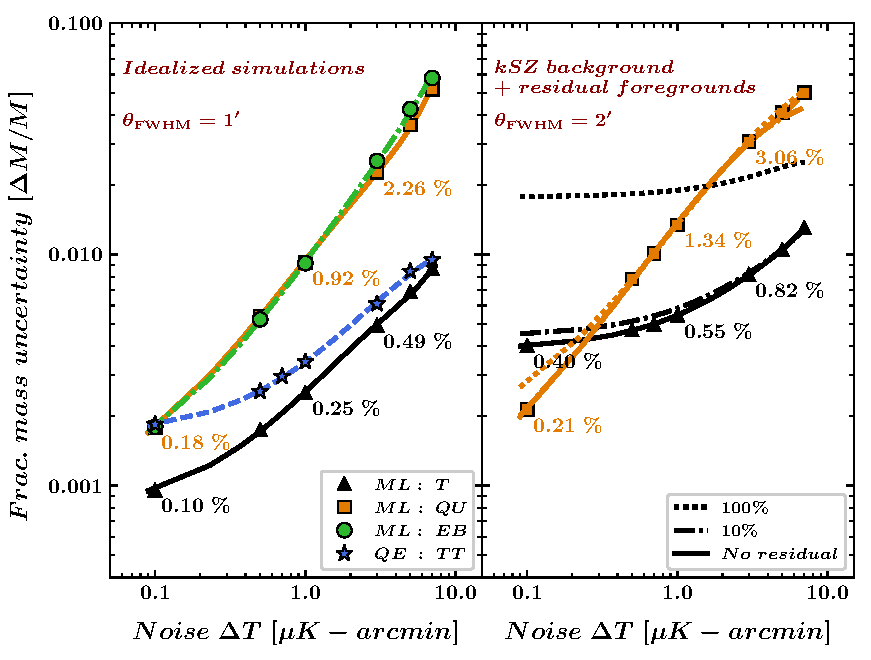
\includegraphics[]{figs/fig1-eps-converted-to.pdf}
 \caption{In the top panel we show the combined likelihood of 100,000 clusters each at redshift of 0.7 and at mass of $2\times 10^{14} M_{\odot}$ for temperature and polarisation MLE estimators. The difference between QU and EB estimator isn't statistically significant. In the bottom panel we show the results of null test and as expected the likelihood peaks at zero for all three estimators}
 \end{figure}
   
   \subsection{Effects of astrophysical foregrounds}
   